\documentclass[14pt,a4paper]{extreport}

\usepackage[T2A]{fontenc}
\usepackage[utf8]{inputenc}
\usepackage[english,russian]{babel}
\usepackage{mathptmx}
\usepackage[left=30mm,right=15mm,top=20mm,bottom=20mm]{geometry}
\usepackage{amsmath,amssymb}
\usepackage{booktabs,array}
\usepackage{graphicx}
\usepackage{float}
\usepackage{setspace}
\onehalfspacing
\usepackage[hidelinks]{hyperref}

% Оформление заголовков по образцу: в заголовке главы используется номер,
% а не слово «Глава».
\makeatletter
\renewcommand{\@makeschapterhead}[1]{%
  \vspace*{10pt}%
  {\parindent\z@\raggedright\normalfont\large #1\par\nobreak\vskip 12pt}%
}
\makeatother
\newcommand{\workchapter}[2]{%
  \refstepcounter{chapter}%
  \setcounter{section}{0}%
  \chapter*{#1\quad #2}%
  \addcontentsline{toc}{chapter}{#1\quad #2}%
}
\renewcommand{\contentsname}{Содержание}
\renewcommand{\bibname}{Литература}

\begin{document}

\begin{titlepage}
\begin{center}
  {\large Министерство науки и высшего образования Российской Федерации}\\[4pt]
  {\large Федеральное государственное автономное образовательное учреждение}\\[-1pt]
  {\large высшего образования}\\[4pt]
  {\large\bfseries «КАЗАНСКИЙ (ПРИВОЛЖСКИЙ) ФЕДЕРАЛЬНЫЙ УНИВЕРСИТЕТ»}\\[10pt]
  {\large Институт математики и механики им. Н.И. Лобачевского}\\[4pt]
  {\large Кафедра математической статистики}\\[30pt]
  {\Large\bfseries Курсовая работа}\\[26pt]
  {\Large\bfseries Анализ данных розничной торговли с помощью множественной регрессии}\\[35pt]
  \begin{flushright}
    Студент группы 05-308\\
    Кибардин Максим Олегович\\[18pt]
    «\_\_\_»\_\_\_\_\_\_\_\_\_\_\_ 2026 г.\quad \_\_\_\_\_\_\_\_\_\_\_\_\_\_\_ М.О. Кибардин\\[28pt]
    Научный руководитель\\
    к.н., доцент \\
    «\_\_\_»\_\_\_\_\_\_\_\_\_\_\_\_ 2026 г.\quad \_\_\_\_\_\_\_\_\_\_\_\_\_\_\_ Р.Ф. Салимов
  \end{flushright}
  \vfill
  Казань --- 2026 г.
\end{center}
\end{titlepage}

\tableofcontents
\clearpage

\chapter*{Введение}
\addcontentsline{toc}{chapter}{ВВЕДЕНИЕ}

Цена товара зависит от его характеристик и положения на рынке. Статистическая модель позволяет кратко описать, как цена связана с выбранными характеристиками, и оценить точность таких выводов [1, 2]. В этой работе рассматривается задача анализа данных о розничной торговле.

\textbf{Цель работы} --- провести обоснованную предварительную подготовку данных розничной торговли и с помощью множественной линейной регрессии оценить связи общей цены товара с покупательским спросом, конкурентными ценами и характеристиками товара.

Для достижения цели решаются следующие задачи:
\begin{enumerate}
  \item кратко описать метод наименьших квадратов и способы проверки коэффициентов;
  \item проверить качество данных, обосновать выбор признаков и оценить корреляции и VIF;
  \item сравнить три модели, в каждой из которых используется цена одного конкурента;
  \item оценить множественную модель с тремя ценами конкурентов, числом покупателей, весом и количеством фотографий в карточке;
  \item интерпретировать коэффициенты, p-value, доверительные интервалы и качество модели;
  \item проверить отдельные коэффициенты, совместный вклад цен конкурентов и значимость модели в целом;
  \item указать ограничения анализа.
\end{enumerate}

\textbf{Объект исследования} --- наблюдения за товарами и их ценами в розничной торговле. \textbf{Предмет исследования} --- статистические связи общей цены товара с покупательским спросом, конкурентными ценами, весом и характеристиками карточки товара.

Используется датасет Retail Price: 676 наблюдений по 52 товарам за 2017--2018 годы. Сравниваются три отдельные спецификации, затем оценивается модель со всеми тремя ценами конкурентов. Коэффициенты оцениваются методом наименьших квадратов; стандартные ошибки группируются по товару, поскольку одни и те же товары встречаются в выборке несколько раз.

\workchapter{1.}{Линейная регрессия и статистическая проверка}

\section{Идея модели и метода наименьших квадратов}

Регрессионная модель описывает отклик $y$ через несколько признаков $x_j$ и случайную ошибку [1, 2]:
\begin{equation}
  y_i = \beta_0 + \beta_1x_{i1}+\dots+\beta_kx_{ik}+\varepsilon_i.
\end{equation}
Здесь $i$ --- номер наблюдения, $j$ --- номер признака, $k$ --- общее число признаков, $y_i$ --- отклик для наблюдения $i$, а $x_{ij}$ --- значение признака $j$ в этом наблюдении. $\beta_0$ --- свободный член, $\beta_j$ --- коэффициент при признаке $j$, $\varepsilon_i$ --- часть отклика, не описанная моделью. Коэффициент $\beta_j$ показывает условное изменение среднего отклика при изменении $x_j$ и фиксированных остальных признаках.

Метод наименьших квадратов (МНК) выбирает коэффициенты, при которых сумма квадратов остатков минимальна:
\begin{equation}
  \widehat{\boldsymbol\beta}=\arg\min_{\boldsymbol\beta}\sum_{i=1}^{n}(y_i-\widehat y_i)^2.
\end{equation}
Знак «шляпка» означает оценённую величину: $\widehat y_i$ --- предсказанное моделью значение, а $\widehat{\boldsymbol\beta}$ --- оценки коэффициентов. В матричной записи при полном ранге матрицы признаков $X$ решение имеет вид
\begin{equation}
  \widehat{\boldsymbol\beta}=(X^\top X)^{-1}X^\top y.
\end{equation}
Здесь $X$ --- матрица значений признаков с отдельным столбцом единиц для свободного члена, $y$ --- вектор наблюдаемых откликов, $X^\top$ --- транспонированная матрица, а $^{-1}$ обозначает обратную матрицу. В этой работе отклик $y$ равен натуральному логарифму общей цены. МНК используется во всех сравниваемых спецификациях.

\section{Логарифмические коэффициенты и качество модели}

В используемой модели логарифмируются общая цена и пять непрерывных факторов: число покупателей, цены трёх конкурентов и вес товара. Количество фотографий включено в исходном масштабе. Поэтому коэффициенты при логарифмах можно приближённо интерпретировать как процентное изменение цены при увеличении соответствующего фактора на один процент, если остальные признаки модели не меняются; коэффициент числа фотографий относится к добавлению одной фотографии. Например, коэффициент $0{,}5$ соответствует связи роста признака на 1\% с ростом цены примерно на 0,5\%.

Качество подгонки кратко характеризуется коэффициентом детерминации:
\begin{equation}
  R^2=1-\frac{\sum_i(y_i-\widehat y_i)^2}{\sum_i(y_i-\bar y)^2}.
\end{equation}
Здесь $y_i$ --- наблюдаемое значение отклика, $\widehat y_i$ --- предсказание модели, $\bar y$ --- среднее наблюдаемых значений, а суммирование $\sum_i$ проводится по всем $n$ наблюдениям. Показатель отражает долю разброса отклика в этой выборке, описанную моделью. Высокое значение $R^2$ само по себе не доказывает правильность модели или причинную связь.

\section{Проверка коэффициентов и модели: t- и F-критерии}

Для каждого коэффициента проверяется гипотеза
\begin{equation}
  H_0:\beta_j=0,\qquad H_1:\beta_j\ne 0.
\end{equation}
Нулевая гипотеза означает, что в рамках выбранной модели данные не подтверждают связь отклика с этим признаком. Статистика критерия равна
\begin{equation}
  t_j=\frac{\widehat\beta_j}{\operatorname{SE}_{\mathrm{cluster}}(\widehat\beta_j)}.
\end{equation}
Здесь $\widehat\beta_j$ --- оценка коэффициента, а $\operatorname{SE}_{\mathrm{cluster}}$ --- её кластерная стандартная ошибка. Она учитывает, что строки одного товара могут быть похожи [2]. В расчётах 52 товарные группы; для t-проверок число степеней свободы равно $52-1=51$.

Уровень значимости заранее выбран равным $\alpha=0{,}05$. p-value показывает, насколько необычной была бы полученная статистика при условии, что нулевая гипотеза верна. Если p-value меньше 0,05, нулевая гипотеза отвергается.

Для двусторонней проверки p-value вычисляется через функцию распределения Стьюдента:
\begin{equation}
  p_j=2\left(1-F_{t_{51}}\left(\lvert t_j\rvert\right)\right),
\end{equation}
Здесь $|t_j|$ --- модуль наблюдаемой t-статистики, $u$ --- аргумент функции, а $F_{t_{51}}(u)$ --- вероятность получить значение t-статистики не больше $u$ при нулевой гипотезе и 51 степени свободы. Множитель 2 учитывает обе стороны двусторонней проверки. В ноутбуке p-value берётся из результата \texttt{statsmodels}: \texttt{get\_robustcov\_results} вызывается с параметрами \texttt{cov\_type='cluster'}, \texttt{use\_t=True} и группировкой по \texttt{product\_id}.

95\%-ный доверительный интервал для коэффициента имеет вид
\begin{equation}
  \widehat\beta_j\pm t_{0{,}975;51}\operatorname{SE}_{\mathrm{cluster}}(\widehat\beta_j).
\end{equation}
Здесь знак $\pm$ задаёт нижнюю и верхнюю границы интервала, а $t_{0{,}975;51}$ --- квантиль t-распределения с 51 степенью свободы, для которого вероятность не превысить значение равна 0,975 (справа остаётся 2,5\%). Он задаёт множитель при стандартной ошибке; интервал симметрично строится вокруг оценки коэффициента. Если интервал не содержит ноль, это согласуется с двусторонним тестом на уровне 5\%. В ноутбуке границы вычисляются методом \texttt{conf\_int} кластерного результата.

Скорректированный коэффициент детерминации рассчитывается по формуле
\begin{equation}
  R^2_{\mathrm{adj}}=1-(1-R^2)\frac{n-1}{n-k-1},
\end{equation}
Здесь $n=676$ --- число наблюдений, $k$ --- число регрессоров без константы ($k=6$ для множественной модели и $k=4$ для каждой отдельной), а $n-k-1$ --- остаточное число степеней свободы с учётом константы. В ноутбуке значения $R^2$ и $R^2_{\mathrm{adj}}$ берутся из объекта \texttt{statsmodels} как \texttt{rsquared} и \texttt{rsquared\_adj}.

Совместная гипотеза о нескольких коэффициентах проверяется кластерно-устойчивым F-критерием. Для линейных ограничений используется статистика Вальда
\begin{equation}
  F=\frac{1}{q}(\mathbf A\widehat{\boldsymbol\beta}-\mathbf c)^\top
  \left[\mathbf A\widehat{\mathbf V}_{\mathrm{cluster}}\mathbf A^\top\right]^{-1}
  (\mathbf A\widehat{\boldsymbol\beta}-\mathbf c),
\end{equation}
Здесь $\mathbf A$ --- матрица, задающая проверяемые линейные ограничения, $\mathbf c$ --- вектор значений коэффициентов при нулевой гипотезе, $\widehat{\boldsymbol\beta}$ --- вектор оценок, $\widehat{\mathbf V}_{\mathrm{cluster}}$ --- кластерная ковариационная матрица оценок, а $q$ --- число ограничений (строк матрицы $\mathbf A$). Для трёх цен конкурентов $q=3$, для проверки всех коэффициентов модели $q=6$. Обозначение $\top$ означает транспонирование, а $^{-1}$ --- обращение матрицы. При нулевой гипотезе статистика сопоставляется с F-распределением со степенями свободы $q$ и 51; p-value равно $1-F_{q,51}(F_{\mathrm{набл}})$, где $F_{q,51}(u)$ --- вероятность получить значение не больше $u$, а $F_{\mathrm{набл}}$ --- рассчитанное значение статистики. В ноутбуке статистика и p-value вычисляются методом \texttt{f\_test} кластерно-устойчивого результата \texttt{statsmodels}.

В расширенной модели отдельно проверяется гипотеза о нулевых коэффициентах всех шести факторов и гипотеза о совместном вкладе цен конкурентов. Для первой проверки нулевая гипотеза имеет вид
\begin{equation}
  H_0:\beta_1=\gamma_1=\gamma_2=\gamma_3=\beta_2=\delta=0,
\end{equation}
то есть ни один из шести факторов не связан с откликом в рамках модели. Для второй проверки рассматривается ограничение $H_0:\gamma_1=\gamma_2=\gamma_3=0$. Для обеих проверок используется F-тест на основе кластерной ковариационной матрицы; число степеней свободы равно соответственно $(6,51)$ и $(3,51)$. Если p-value меньше 0,05, соответствующая нулевая гипотеза отвергается. Совместные тесты дополняют, но не заменяют проверку отдельных коэффициентов.

\workchapter{2.}{Анализ данных розничной торговли с помощью множественной регрессии}

\section{Данные и выбор признаков}

В используемом файле данных Retail Price [3] содержатся 676 строк, 30 столбцов и 52 товара, наблюдаемых в разные месяцы 2017--2018 годов. В исходной таблице нет пропусков, полных дубликатов и повторов пары «товар--месяц». Для переменных итоговой модели нет нулевых или отрицательных значений, поэтому после проверок все 676 наблюдений сохранены. Автоматического удаления крайних значений не проводилось: без подтверждения ошибки ввода они могут быть реальными наблюдениями.

Набор факторов выбран по вопросу исследования и содержательной роли переменных: число покупателей служит показателем спроса, цены всех трёх конкурентов описывают конкурентную среду, вес отражает физическую характеристику товара, а число фотографий включено как контроль полноты карточки. Последний признак не выбран по статистической значимости: его коэффициент в итоговой модели незначим. В 95\% строк относительное расхождение между \texttt{total\_price} и произведением \texttt{unit\_price} на \texttt{qty} не превышает 0,283\%; поэтому эти два показателя не включаются как регрессоры, чтобы не описывать целевую переменную почти через её собственные составляющие. Корреляция \texttt{unit\_price} и \texttt{lag\_price} равна 0,994; близкие ценовые показатели не включаются одновременно. Признак \texttt{s} исключён, поскольку его смысл в описании неоднозначен.

В модель включено число фотографий \texttt{product\_photos\_qty} как контрольная характеристика карточки (от 1 до 8). \texttt{freight\_price} отражает отдельную стоимость доставки, не включённую в \texttt{total\_price}; в ней есть одно нулевое значение, поэтому логарифмировать её без дополнительного преобразования нельзя. Девять категорий товара потребовали бы восьми индикаторных признаков. Проверка \texttt{product\_score} и \texttt{volume} по отдельности не повысила скорректированный $R^2$ (p-value 0,938 и 0,712), поэтому эти признаки оставлены за рамками компактной спецификации. Календарные переменные потребовали бы отдельной модели временных эффектов. Крайние значения не удаляются только по статистическому порогу.

Для шести регрессоров рассчитаны парные корреляции и факторы инфляции дисперсии (VIF). Максимальная абсолютная парная корреляция равна 0,582. Значения VIF находятся в диапазоне 1,055--1,839: это ниже часто используемого ориентировочного порога 5, поэтому оснований удалять включённые факторы по причине выраженной мультиколлинеарности нет. Число фотографий сохраняется как контроль по содержательному основанию, хотя его индивидуальный коэффициент незначим ($p=0{,}154$). Порог VIF является диагностической эвристикой, а не строгим критерием.

Для отдельного регрессора VIF определяется через вспомогательную регрессию этого регрессора на остальные факторы:
\begin{equation}
  \operatorname{VIF}_j=\frac{1}{1-R_j^2}.
\end{equation}
Здесь $j$ --- номер регрессора, а $R_j^2$ --- коэффициент детерминации вспомогательной регрессии, в которой этот регрессор объясняется всеми остальными включёнными факторами. Чем лучше остальные факторы предсказывают $x_j$, тем выше VIF. В ноутбуке он вычисляется функцией \texttt{variance\_inflation\_factor} из \texttt{statsmodels}; матрица парных корреляций строится методом \texttt{DataFrame.corr()}.

Краткие характеристики переменных приведены в Таблице~\ref{tab:description}. Средняя общая цена заметно выше медианной, что указывает на возможную правостороннюю асимметрию. Логарифмическая форма также упрощает интерпретацию коэффициентов как эластичностей.

На Рисунке~\ref{fig:price_distribution} показано распределение общей цены до и после логарифмирования. На исходной шкале заметен правый хвост, а логарифмирование сжимает большие значения. График помогает описать распределение и выбранное преобразование, но сам по себе не доказывает корректность модели.

\begin{figure}[H]
  \centering
  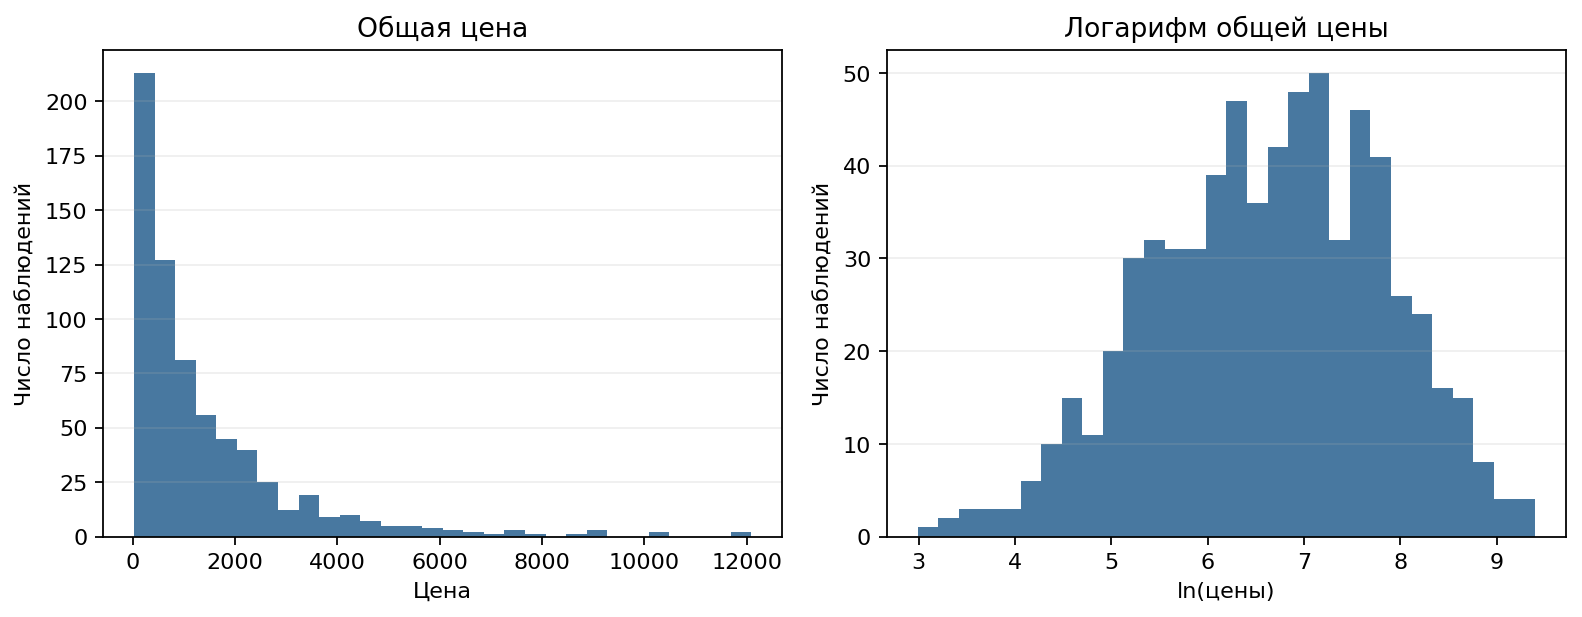
\includegraphics[width=0.92\textwidth]{price_distribution_simple.png}
  \caption{Распределение общей цены и её натурального логарифма}
  \label{fig:price_distribution}
\end{figure}

\begin{table}[H]
  \centering
  \caption{Описательная статистика исходных переменных}
  \label{tab:description}
  \small
    \begin{tabular}{lrrrr}
    \toprule
    Переменная & Среднее & Медиана & Минимум & Максимум \\
    \midrule
    Общая цена & 1422,71 & 807,89 & 19,90 & 12095,00 \\
    Число покупателей & 81,03 & 62,00 & 1,00 & 339,00 \\
    Цена конкурента 1 & 79,45 & 69,90 & 19,90 & 349,90 \\
    Цена конкурента 2 & 92,93 & 89,99 & 19,90 & 349,90 \\
    Цена конкурента 3 & 84,18 & 59,90 & 19,90 & 255,61 \\
    Вес товара, г & 1847,50 & 950,00 & 100,00 & 9750,00 \\
    Число фотографий & 1,99 & 1,50 & 1,00 & 8,00 \\
    \bottomrule
  \end{tabular}
\end{table}

Для краткой оценки взаимосвязи рассчитаны парные корреляции Пирсона между логарифмированными ценами конкурентов (Таблица~\ref{tab:correlations}). Корреляции умеренные; при совместном включении этих переменных важно отличать их отдельные связи от совместного результата. Попарная корреляция показывает только связи двух признаков; поэтому её дополняет расчёт VIF для всех шести регрессоров.

\begin{table}[H]
  \centering
    \caption{Парные корреляции логарифмированных цен конкурентов}
  \label{tab:correlations}
  \small
    \begin{tabular}{lrrr}
    \toprule
    Признак & Цена конкурента 1 & Цена конкурента 2 & Цена конкурента 3 \\
    \midrule
    Цена конкурента 1 & 1,0000 & 0,4358 & 0,5815 \\
    Цена конкурента 2 & 0,4358 & 1,0000 & 0,5117 \\
    Цена конкурента 3 & 0,5815 & 0,5117 & 1,0000 \\
    \bottomrule
  \end{tabular}
\end{table}

В Таблице~\ref{tab:vif} приведены VIF всех регрессоров итоговой модели. Все значения заметно ниже ориентировочного уровня 5; поэтому выбранные факторы сохранены.

\begin{table}[H]
  \centering
  \caption{Факторы инфляции дисперсии регрессоров модели}
  \label{tab:vif}
  \small
  \begin{tabular}{lr}
    \toprule
    Фактор & VIF \\
    \midrule
    Число покупателей & 1,055 \\
    Цена конкурента 1 & 1,839 \\
    Цена конкурента 2 & 1,495 \\
    Цена конкурента 3 & 1,755 \\
    Вес товара & 1,152 \\
    Число фотографий & 1,063 \\
    \bottomrule
  \end{tabular}
\end{table}

\section{Спецификация модели}

Чтобы сравнить цены конкурентов при одинаковых контрольных признаках, сначала оцениваются три отдельные модели. Для каждой цены конкурента $j=1,2,3$ используется спецификация
\begin{equation}
\begin{aligned}
\ln(\texttt{total\_price}_i) ={}& \beta_0+\beta_1\ln(\texttt{customers}_i)\\
&+\gamma_j\ln(\texttt{comp\_j}_i)+\beta_2\ln(\texttt{product\_weight\_g}_i)\\
&+\delta\,\texttt{product\_photos\_qty}_i+\varepsilon_i.
\end{aligned}
\end{equation}
Затем оценивается расширенная модель, в которой все три цены учитываются одновременно:
\begin{equation}\label{eq:model}
\begin{aligned}
\ln(\texttt{total\_price}_i) ={}& \beta_0+\beta_1\ln(\texttt{customers}_i)\\
&+\gamma_1\ln(\texttt{comp\_1}_i)+\gamma_2\ln(\texttt{comp\_2}_i)\\
&+\gamma_3\ln(\texttt{comp\_3}_i)+\beta_2\ln(\texttt{product\_weight\_g}_i)\\
&+\delta\,\texttt{product\_photos\_qty}_i+\varepsilon_i.
\end{aligned}
\end{equation}
Здесь $\ln$ --- натуральный логарифм, $\beta_0$ --- свободный член, $\beta_1$ --- коэффициент числа покупателей, $\gamma_j$ --- коэффициент цены конкурента $j$, $\beta_2$ --- коэффициент веса, $\delta$ --- коэффициент количества фотографий, а $\varepsilon_i$ --- остаток для наблюдения $i$. Коэффициенты при пяти логарифмированных признаках приблизительно интерпретируются как эластичности; $\delta$ относится к добавлению одной фотографии. Во всех спецификациях используются одни и те же 676 наблюдений. Стандартные ошибки кластеризуются по 52 товарам. Скорректированный $R^2$ сравнивает подгонку трёх отдельных моделей в этой выборке; он не является оценкой точности прогноза на новых данных.

\section{Результаты}

В Таблице~\ref{tab:candidate_models} приведены три модели с ценой одного конкурента; во всех также учтены покупатели, вес и число фотографий. Все три оценки положительны и значимы при 5\%. Наибольший скорректированный $R^2$ у спецификации с ценой второго конкурента; это лучшая подгонка в данной выборке, но не проверка прогноза на новых данных.

\begin{table}[H]
  \centering
  \caption{Сравнение отдельных моделей с разными ценами конкурентов}
  \label{tab:candidate_models}
  \small
  \begin{tabular}{lrrrr}
    \toprule
    Конкурент & $\widehat\gamma_j$ & p-value & 95\%-ный кластерный интервал & Скорр. $R^2$ \\
    \midrule
    Первый & 0,371 & 0,0121 & [0,085; 0,656] & 0,239 \\
    Второй & 0,724 & $2{,}74\cdot10^{-6}$ & [0,448; 0,999] & 0,299 \\
    Третий & 0,539 & $8{,}70\cdot10^{-4}$ & [0,233; 0,845] & 0,258 \\
    \bottomrule
  \end{tabular}
\end{table}

Далее рассматривается множественная модель~\eqref{eq:model}, где каждая оценка конкурента отражает условную связь при фиксации двух других цен, покупателей, веса и числа фотографий. В Таблице~\ref{tab:full_results} представлены двусторонние t-проверки, p-value и 95\%-ные кластерные доверительные интервалы.

\begin{table}[H]
  \centering
  \caption{Результаты расширенной модели со всеми ценами конкурентов}
  \label{tab:full_results}
  \small
  \begin{tabular}{lrrrrr}
    \toprule
    Признак & Коэффициент & SE & $t$ & p-value & 95\%-ный интервал \\
    \midrule
    Число покупателей & 0,550 & 0,060 & 9,16 & $2{,}39\cdot10^{-12}$ & [0,430; 0,671] \\
    Цена конкурента 1 & 0,024 & 0,134 & 0,18 & 0,856 & [$-0{,}244$; 0,293] \\
    Цена конкурента 2 & 0,594 & 0,188 & 3,16 & 0,0027 & [0,216; 0,971] \\
    Цена конкурента 3 & 0,224 & 0,202 & 1,11 & 0,274 & [$-0{,}183$; 0,630] \\
    Вес товара & 0,152 & 0,059 & 2,59 & 0,0124 & [0,034; 0,270] \\
    Число фотографий & 0,100 & 0,069 & 1,45 & 0,154 & [$-0{,}039$; 0,240] \\
    \bottomrule
  \end{tabular}
\end{table}

В множественной модели после одновременного учёта трёх цен конкурентов индивидуальная положительная связь сохраняется для цены второго конкурента ($p=0{,}0027$). Для первого и третьего конкурентов доверительные интервалы включают ноль. Число фотографий также незначимо отдельно ($p=0{,}154$); включение его как контрольного признака не является утверждением о подтверждённом эффекте.

Совместный кластерно-устойчивый тест коэффициентов трёх цен конкурентов даёт $F(3,51)=11{,}24$ и $p=8{,}98\cdot10^{-6}$. Цены конкурентов значимы совместно. Тест всех шести коэффициентов также значим: $F(6,51)=23{,}98$, $p=2{,}91\cdot10^{-13}$.

Коэффициент детерминации множественной модели равен $R^2=0{,}311$, скорректированный $R^2=0{,}305$. Модель описывает около 31,1\% разброса логарифма цены в этой выборке.

Для наглядной интерпретации при росте признака на 10\% модельная процентная оценка рассчитывается как $(\left(1{,}10\right)^{\widehat{\beta}}-1)\cdot100\%$. При прочих равных она составляет около 5,4\% для числа покупателей, 5,8\% для цены второго конкурента и 1,5\% для веса. Число фотографий интерпретируется на одну фотографию; его коэффициент незначим, поэтому точечную оценку не следует представлять как подтверждённую связь. Интервалы для \texttt{comp\_1} и \texttt{comp\_3} также включают ноль.

На Рисунке~\ref{fig:coefficients} оценки шести факторов показаны с 95\%-ными кластерными доверительными интервалами; вертикальная линия соответствует нулю.

\begin{figure}[H]
  \centering
  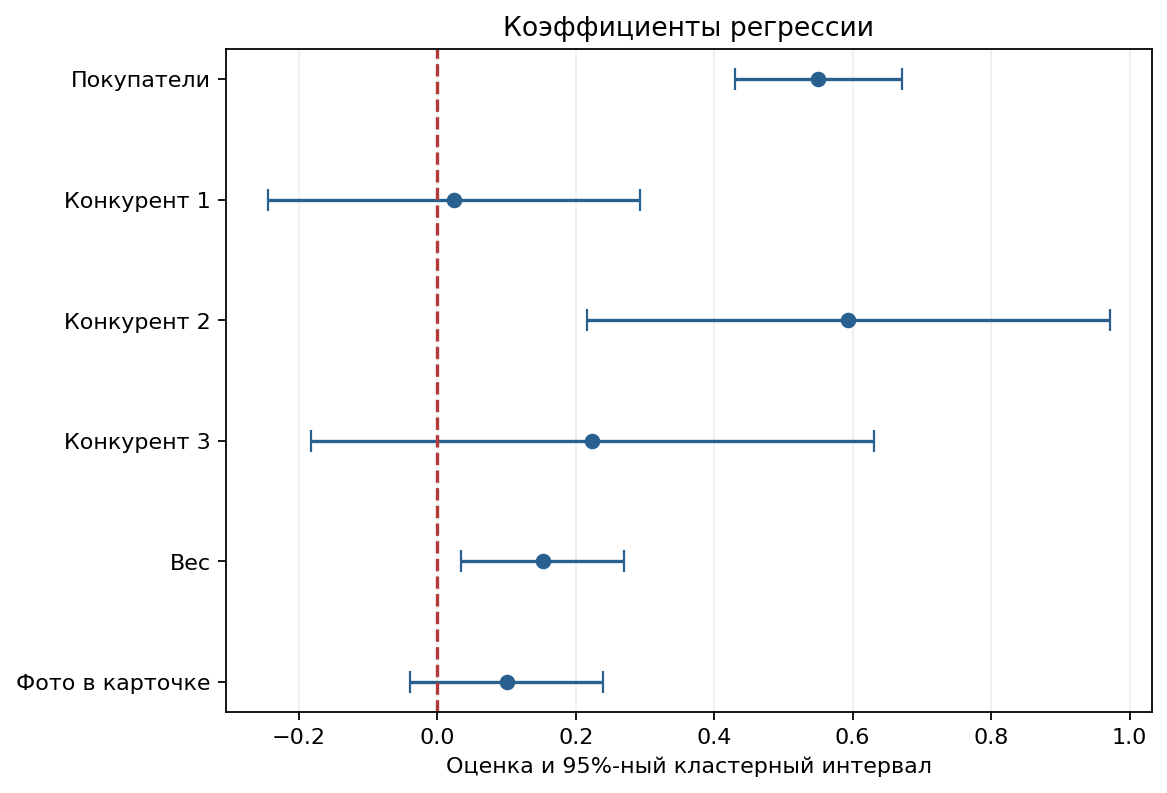
\includegraphics[width=0.78\textwidth]{coefficients_ci_simple.png}
  \caption{Оценки коэффициентов и 95\%-ные кластерные доверительные интервалы}
  \label{fig:coefficients}
\end{figure}

\section{Краткая проверка модели и ограничения}

На Рисунке~\ref{fig:residuals} показаны остатки модели в зависимости от предсказанных значений. Точки расположены по обе стороны от нулевой линии, однако разброс остатков неодинаков и присутствуют отдельные большие отклонения. График служит краткой визуальной проверкой и не заменяет формальные диагностические тесты.

\begin{figure}[H]
  \centering
  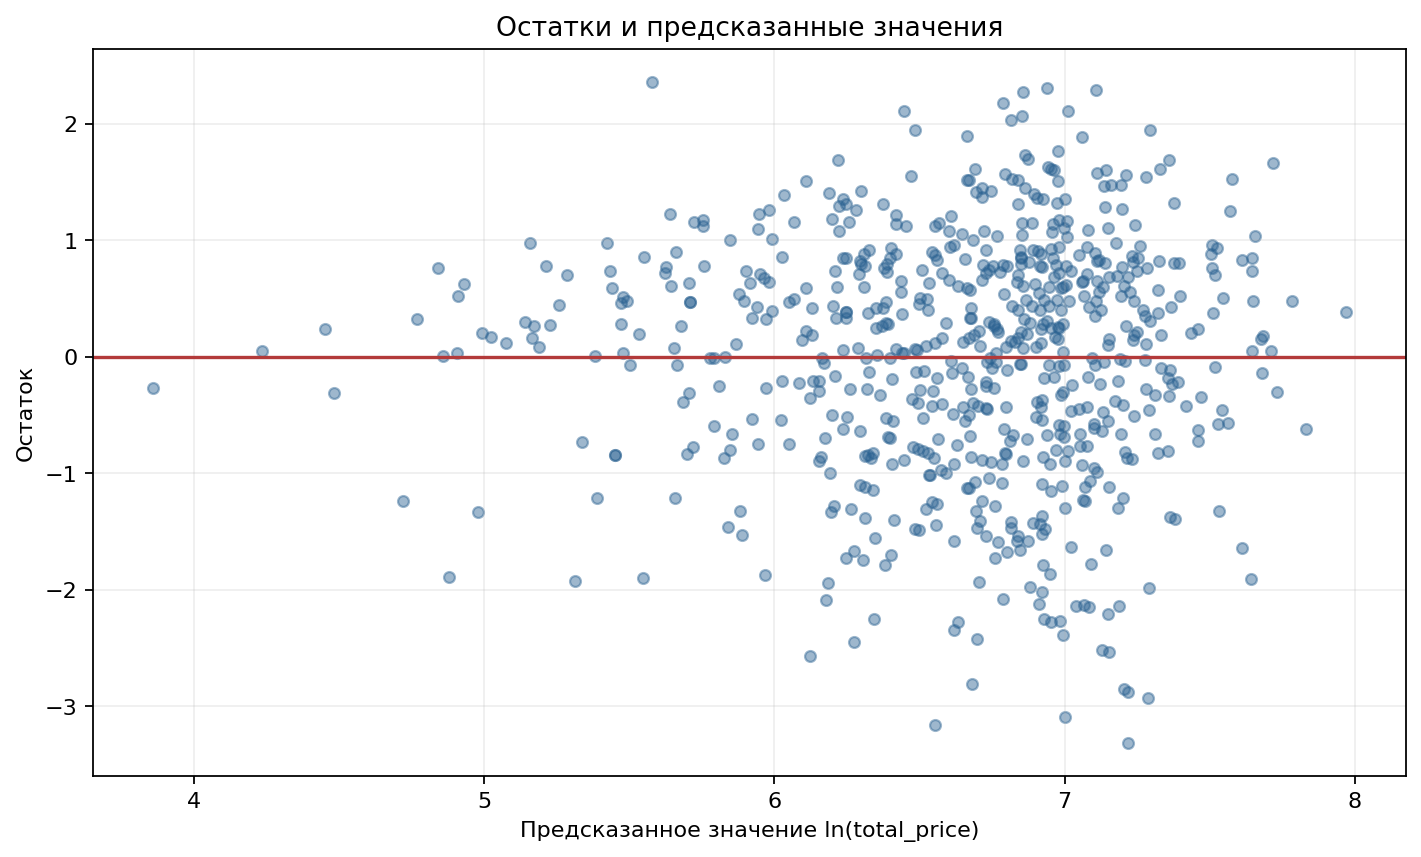
\includegraphics[width=0.92\textwidth]{residuals_simple.png}
  \caption{Остатки модели и предсказанные значения логарифма цены}
  \label{fig:residuals}
\end{figure}

У исследования есть несколько ограничений. Во-первых, наблюдательные данные позволяют говорить о связи, но не о причинном влиянии. Во-вторых, модель включает шесть факторов, но не учитывает категории товаров, сезонность и другие возможные характеристики. В-третьих, сравнение спецификаций выполнено на той же выборке и не является проверкой точности прогноза на новых товарах. Кластерные стандартные ошибки учитывают повторные наблюдения по одному товару при оценке неопределённости, но не устраняют возможное влияние неучтённых характеристик товаров.

\chapter*{Заключение}
\addcontentsline{toc}{chapter}{ЗАКЛЮЧЕНИЕ}

В работе проверено качество данных: пропусков, полных дубликатов и повторов «товар--месяц» нет, все 676 наблюдений сохранены. Обоснован выбор шести регрессоров и объяснено исключение других столбцов. Сравнивались три модели с ценой одного конкурента и числом фотографий, затем оценивалась множественная модель со всеми ценами конкурентов. Стандартные ошибки сгруппированы по товару; приведены t-проверки, p-value и 95\%-ные интервалы.

В отдельных моделях все цены конкурентов положительны и значимы; наибольший скорректированный $R^2$ у \texttt{comp\_2}. В множественной модели индивидуально значима цена второго конкурента, а все три конкурентные цены значимы совместно. Также значимы число покупателей и вес. Число фотографий включено как контроль, но его отдельная связь не подтверждена. $R^2=0{,}311$, скорректированный $R^2=0{,}305$.

Совместный тест шести коэффициентов ($F(6,51)=23{,}98$, $p<0{,}001$) и тест трёх цен конкурентов ($F(3,51)=11{,}24$, $p<0{,}001$) подтверждают значимость соответствующих групп факторов, но не каждого конкурента по отдельности.

Итак, в этой выборке цена второго конкурента показывает наиболее ясную индивидуальную связь с общей ценой после учёта других факторов. Результаты остаются статистическими связями, а не доказательством причинного влияния; для более широких выводов нужны дополнительные данные и проверка на новых наблюдениях.

\chapter*{Литература}
\addcontentsline{toc}{chapter}{ЛИТЕРАТУРА}

\begin{enumerate}
  \item Кобзарь А.И. Прикладная математическая статистика. --- М.: Физматлит, 2006.
  \item Wooldridge J.M. Introductory Econometrics: A Modern Approach. --- 6th ed. --- Cengage Learning, 2016.
  \item Retail Price Optimization. Набор данных. Kaggle. URL: \url{https://www.kaggle.com/datasets/suddharshan/retail-price-optimization} (дата обращения: 22.10.2026).
\end{enumerate}

\end{document}
